% !TeX spellcheck = cs_CZ
{\tikzset{external/prefix={tikz/FYZI/}}
 \tikzset{external/figure name/.add={ch12_}{}}
%---------------------------------------------------------------------------------------------------
% file fey1ch15.tex
%---------------------------------------------------------------------------------------------------
%============================= Kapitola: Speciální teorie relativity ===============================
\chapter{Speciální teorie relativity}\label{fyz:IchapXV}
\minitoc

  \section{Princip relativity}\label{fyz:IchapXVsecI}
    Více než \num{200} let se věřilo, že Newtonovy rovnice správně popisují přírodu. Když se v nich 
    poprvé našla chyba, našel se i způsob, jak jej odstranit. Oboje, chybu i korekci, objevil 
    \textbf{Einstein} v roce \num{1905}.
    
    V druhém Newtonově zákoně, daném vztahem 
    \begin{equation*}
      F = \der{(mv)}{t}
    \end{equation*}
    se mlčky předpokládalo, že \(m\) je konstantní veličina. Ale nyní víme, že to není pravda a že 
    hmotnost tělesa roste, zvyšuje-li se jeho rychlost. V Einsteinově opraveném vztahu má \(m\) 
    hodnotu 
    \begin{equation}\label{FYZ:eq182}
      m = \frac{m_0}{\sqrt{1-\frac{v^2}{c^2}}}
    \end{equation}  
    kde \(m_0\) je \emph{klidová hmotnost} (hmotnost tělesa, jež se nepohybuje) a $c$ je 
    \emph{rychlost světla}, která je přibližně rovna $3\cdot10^5\, km\cdot s^{-1}$.
    
    Ze vztahu je vidět, že za normálních okolností je přírůstek hmotnosti velmi malý. Dokonce i pro 
    družici Země, jež se pohybuje rychlostí \SI{9.0}{\km\per\s} je \(v/c = \num{3e-5}\) a po 
    dosazení do uvedeného vztahu dostaneme korekci hmotnosti ne větší než dvě až tři miliardtiny, 
    což téměř nelze pozorovat. Platnost vztahu však byla dostatečně potvrzena pozorováním mnoha 
    druhů částic, jejichž rychlosti dosahují prakticky až rychlosti světla. Za normálních okolností 
    je tento efekt velmi malý a proto je pozoruhodné, že byl objeven nejprve teoreticky a až potom 
    experimentálně. Proto je zajímavé sledovat, jaké kombinace experimentů a fyzikálních úvah vedla 
    k odhalení tak jemné modifikace zákona. Přispělo k tomu nemálo lidí, přičemž konečným výsledkem 
    byl Einsteinův objev.
    
    Existují dvě Einsteinovy teorie relativity. Tato kapitola hovoří o \emph{speciální teorii 
    relativity} z roku \num{1905}. V roce \num{1915} uveřejnil Einstein dodatečnou teorii nazvanou 
    \emph{Obecná teorie relativity}. Ta je zobecněním speciální teorie relativity pro případ 
    \emph{gravitace}.
         
    Newton byl první, kdo vyslovil \emph{princip relativity} jako jeden z důsledků pohybových 
    zákonů: Vzájemné pohyby těles, nacházejících se v daném prostoru, jsou stejné ať je prostor v 
    klidu, nebo se pohybuje rovnoměrně přímočaře vpřed. To například znamená, že jestliže se 
    kosmická loď pohybuje rovnoměrnou rychlostí, všechny experimenty a všechny jevy v lodi budou 
    probíhat tak, jakoby se loď nepohybovala (samozřejmě za předpokladu, že se nikdo nebude dívat 
    ven). To je smyslem principu relativity. Myšlenka je jednoduchá, jedinou otázkou je, zda je 
    pravda, že ve všech experimentech provedených v pohybující se soustavě budou všechny fyzikální 
    zákony stejné, jako v soustavě, která je v klidu. Nejprve zjistíme, zda v pohybující se
    soustavě mají Newtonovy zákony stejný tvar.
    
    \begin{figure}[ht!]  %\ref{fyz:fig005}
      \centering
      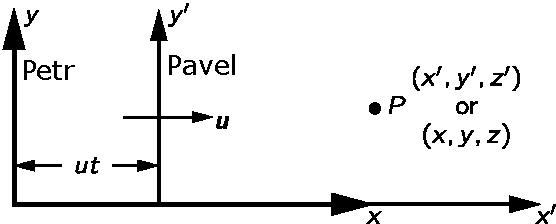
\includegraphics[width=0.7\linewidth]{fyz_fig005.pdf}
      \caption{Dvě souřadnicové soustavy v rovnoměrném relativním pohybu podél svých x-ových os.
               (\cite[s.~211]{Feynman01})}
      \label{fyz:fig005}
    \end{figure}
    
    Předpokládejme, že se Pavel pohybuje konstantní rychlostí \(u\) ve směru osy \(x\), přičemž 
    měří polohu určitého budu (obr. \ref{fyz:fig005}). Ve své souřadnicové soustavě si 
    značí souřadnici ve směru osy \(x\) jako \(x'\). Petr je v klidu, přičemž měří polohu téhož 
    bodu. Souřadnici ve směru osy \(x\) ve své souřadnicové soustavě značí jako \(x\). Počátek 
    souřadnicové soustavy, v níž je Pavel, se posune za čas \(t\) o vzdálenost \(ut\), a jestliže 
    soustavy z počátku splývaly, máme
    \begin{equation}\label{FYZ:eq183}
      x' = x - ut, \quad y' = y, \qquad z' = z, \quad t' = t. 
    \end{equation}
    Dosadíme-li tuto transformaci do Newtonových zákonů, zjistíme, že se přetransformovaly do 
    stejných zákonů v čárkované soustavě. To znamená, že Newtonovy zákony mají stejný tvar v 
    pohybující se soustavě jako v stacionární soustavě, a proto na základě mechanických experimentů 
    není možné říci, zda se soustava pohybuje či nikoliv. 
    
    Zájem o tento princip vzrostl v minulém století v důsledku výzkumu elektrických, magnetických a 
    světelných jevů, jež vyústilo v \emph{Maxwellovu teorii elektromagnetického pole}, která 
    jednotně popisuje elektřinu, magnetizmus a světlo. Zdálo se však, že Maxwellovy rovnice 
    nevyhovovaly \emph{principu relativity}, neboť přetransformujeme-li Maxwellovy rovnice pomocí 
    rovnic \ref{FYZ:eq183}, nebudou mít stejný tvar. Proto by se elektrické a optické jevy 
    v letící kosmické lodi měli lišit od jevů v nehybné lodi. Těmito jevy by pak bylo možné určit 
    rychlost lodi, a ve speciálním případě pomocí vhodných optických nebo elektrických měření by 
    bylo možné určit i absolutní rychlost lodi. Jedním z důsledků Maxwellových rovnic je, že 
    dojde-li k určité poruše pole, při níž vniká světlo, toto elektromagnetické vlnění se šíří 
    všemi směry stejnou rychlostí \(c = \SI{3e5}{\km\per}\). Dalším důsledkem těchto rovnic 
    je, že pohybuje-li se zdroj poruchy, šíří se vyzářené světlo prostorem stejnou rychlostí \(c\). 
    Tato nezávislost pohybu vlnění na pohybu zdroje vede k zajímavému problému:
    
    Předpokládejme, že sedíme v autě, jež jede rychlostí \(u\) a že světlo z reflektorů auta za 
    námi nás míjí rychlostí \(c\). Zdiferencováním první rovnice \ref{FYZ:eq183} máme
    \begin{equation}\label{FYZ:eq184}
      \der{x'}{t} =\der{x}{t} - u, 
    \end{equation}       
    což znamená, že podle \emph{Galileovy transformace} by zdánlivá rychlost světla měřená z auta 
    nemohla být \(c\), ale \(c-u\). Na této myšlence bylo založeno mnoho experimentů k určení 
    rychlosti Země, ale všechny selhaly - nedávaly vůbec žádné rychlosti. Ukázalo se, že někde 
    \emph{byla} chyba, a sice něco nebylo v pořádku s fyzikálními rovnicemi. Co to asi mohlo být?

  %----------------------- Lorentzova transformace -------------------------------------------------
  \section{Lorentzova transformace}\label{fyz:IchapXVsecII}
    Když se zjistilo, že s rovnicemi v uvedeném případě není vše v pořádku, nejprve padlo podezření 
    na Maxwellovy rovnice elektrodynamiky, jež byly tehdy známy jen dvacet let. Zdálo se být téměř 
    samozřejmé, že tyto rovnice musí byt nesprávné a proto byla snaha je změnit tak, aby při 
    Galileiho transformaci zachovávaly princip relativity. Přitom bylo třeba do těchto rovnic 
    zavést nové členy, jež vedly k předpovědi nových elektrických jevů, jejichž existence se 
    experimentálně nepotvrdila. Proto bylo třeba tuto cestu opustit. Postupně se pak stalo zřejmým, 
    že Maxwellovy zákony elektrodynamiky jsou správné a zdroj problému je třeba hledat někde 
    jinde.  
    
    Mezitím si \emph{H. A. Lorentz} všiml pozoruhodné věci, když použil v Maxwellových rovnicích substituci
    \begin{equation}\label{FYZ:eq185}
      x' = \frac{x - ut}{\sqrt{1-\dfrac{u^2}{c^2}}}, \quad
      y' = y, \quad z' = z,                         \quad
      t' = \frac{t-\dfrac{u}{c^2}x}{\sqrt{1-\dfrac{u^2}{c^2}}}. 
    \end{equation} 
    tvar rovnic se nezměnil. Rovnice \ref{FYZ:eq185} jsou známé jako \emph{Lorentzovy 
    transformace}. Einstein sledoval původní \emph{Poincarého} myšlenku a pak navrhl, že všechny 
    fyzikální zákony, by měly být takové, aby se při Lorentzově transformaci neměnily. Jinými 
    slovy, měly bychom změnit ne zákony elektrodynamiky, ale zákony mechaniky. Jak se ukázalo 
    jediné co je třeba, je změnit hmotnost \(m\) v Newtonových rovnicích podle vztahu 
    \ref{FYZ:eq182}. Po této změně budou Newtonovy zákony v souladu se zákony elektrodynamiky. Když 
    k porovnání Pavlových a Petrových měření použijeme Lorentzovu transformaci, nikdy nebudeme 
    schopni zjistit, zda se jeden nebo druhý pohybuje, neboť tvary všech rovnic budou v obou 
    souřadnicových soustavách stejné. 
    
    Pro pochopení smyslu této nové transformace nestačí studovat jen zákony mechaniky, ale podobně 
    jako Einstein, musíme provést analýzu našeho chápání prostoru a času. 
  
  \section{Michelson-Morleyův experiment}\label{fyz:IchapXVsecIII}
    Jak jsme již zmínili, prováděly se pokusy určit absolutní rychlost Země v hypotetickém „éteru“, 
    o němž se předpokládalo, že je jím prostoupen celý prostor. Nejznámější z těchto experimentů je 
    experiment, jež provedli \emph{Michelson} a \emph{Morley} v roce \num{1887}. Bylo to o \num{18} 
    let dříve, než se konečně Einsteinovi podařilo podat vysvětlení negativních výsledků tohoto 
    pokusu.

    Michelsonův-Morleyho experiment byl proveden pomocí přístroje, jehož schéma je na obr. 
    \ref{fyz_fig004}. Přístroj se skládal ze zdroje světla \(A\), polopropustného postříbřeného 
    zrcadla \(B\) a dvou zrcadel \(C\) a \(E\), vše namontováno na pevné základně. Zrcadla jsou 
    vzdálena od \(B\) ve stejných vzdálenostech \(L\). Dopadající paprsek světla se na 
    polopropustném zrcadle \(B\) rozdvojí a takto rozdvojené paprsky letí k zrcadlům po navzájem 
    kolmých dráhách, odkud se odrážejí zpět k bodu \(B\). Po dopadu na \(B\) se paprsky opět spojí 
    jako superpozice dvou paprsků \(D\) a \(F\). Proletí-li světlo z \(B\) do \(E\) a zpět za 
    stejnou dobu jako z \(B\) do \(C\) a zpět, budou vyletující paprsky \(F\) a \(D\) ve fázi a 
    navzájem se zesílí, ale jestliže se tyto dvě doby trochu liší, nebudou paprsky ve fázi a 
    vznikne interference. Nachází-li se přístroj vzhledem k éteru v „klidu“, doby letu paprsků by 
    se měly navzájem přesně rovnat, ale pohybuje-li se vpravo rychlostí \(u\), měly by být doby 
    rozdílné. Podívejme se proč.
    
    Nejprve vypočtěme dobu, kterou potřebuje světlo k letu z \(B\) do \(E\) a zpět. Řekněme, že 
    doba letu od polopropustného zrcadla \(B\) k zrcadlu \(E\) je \(t_1\) a čas letu zpět je 
    \(t_2\). Zatímco světlo letí z \(B\) do \(E\) přístroj se posune o vzdálenost \(ut_1\), takže 
    světlo muselo proletět rychlostí \(c\) vzdálenost \(L + ut_1\). Tuto vzdálenost lze vyjádřit 
    jako \(ct_1\), takže máme    
    \begin{equation*}
      ct_1 = L + ut_1, \qquad\text{tj.}\quad t_1 = \frac{L}{c - u}.
    \end{equation*}
    I tento výsledek je zřejmý, neboť relativní rychlost světla vzhledem k přístroji je \(c – u\), 
    takže doba je rovna vzdálenosti \(L\) dělené rychlostí \(c- u\). Podobně můžeme vypočítat dobu 
    \(t_2\). O tuto dobu se zrcadlo \(B\) posune o vzdálenost \(ut_2\) a zpáteční dráha světlaje 
    rovna \(L- ut_2\). Takže máme
    \begin{equation*}
      ct_2 = L - ut_2, \qquad\text{tj.}\quad t_2 = \frac{L}{c + u}.
    \end{equation*}
    
    \begin{figure}[ht!]  %\ref{fyz_fig004}
      \centering
      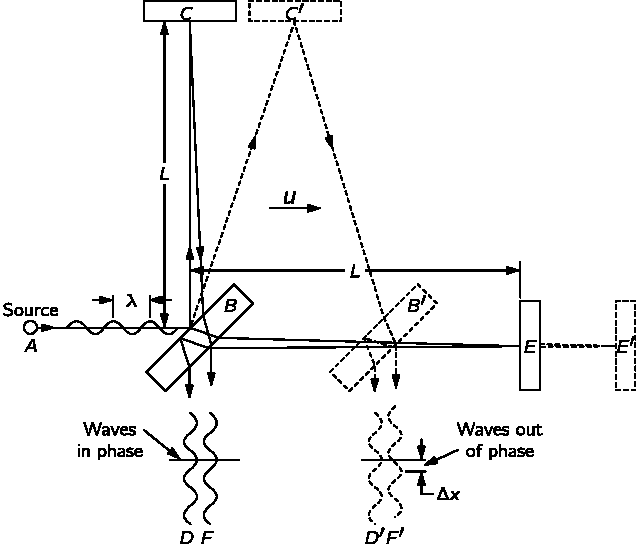
\includegraphics[width=0.99\linewidth]{fyz_fig004.pdf}
      \caption{Schématický náčrt Michelsonova-Morleyova experimentu (\cite[s.~214]{Feynman01})}
      \label{fyz_fig004}
    \end{figure} 
    
    \begin{align}
      \shortintertext{Celková doba je pak}
        t_1 + t_2 &= \frac{2L}{c^2 - u^2},                            \nonumber\\
      \shortintertext{což je vhodné zapsat ve tvaru}
        t_1 + t_2 &= \frac{\dfrac{2L}{c}}{1- \dfrac{u^2}{c^2}}.       \label{FYZ:eq186}
    \end{align}
    
    Nyní vypočteme dobu \(t_3\), během níž proletí světlo vzdálenost od zrcadla \(B\) k zrcadlu 
    \(C\) Podobně jako předtím za dobu \(t_3\) se bude zrcadlo \(C\) pohybovat vpravo na vzdálenost 
    \(ut_3\) do bodu \(C\). Současně s tím projde světlo vzdálenost \(ct_3\) podél přepony 
    trojúhelníka, kterou tvoří \(BC'\). Pro tento pravoúhlý trojúhelník platí
    \begin{equation*}
      (ct_3)^2=L^2+(ut_3)^2  \quad\text{neboli}\quad L^2=c^2t_3^2−u^2t_3^2=(c^2−u^2)t_3^2,
    \end{equation*}
    odkud máme
    \begin{equation*}
      t_3=\frac{L}{\sqrt{c^2−u^2}}.
    \end{equation*}
    Na zpáteční cestě proletí světlo stejnou vzdálenost, což je vidět ze symetrie nákresu, takže i 
    doba návratu je stejná a celková doba je rovna \(2t_3\). Po malých úpravách můžeme psát
    \begin{equation}\label{FYZ:eq187}
      2t_3=\frac{2L}{c^2−u^2} = \frac{\dfrac{2L}{c}}{\sqrt{1−\dfrac{u^2}{c^2}}}
    \end{equation}
    Nyní můžeme porovnat doby obou paprsků. Čitatele ve výrazech (\ref{FYZ:eq186}) a 
    (\ref{FYZ:eq187}) jsou stejné a představují dobu letu paprsků, kdyby byl přístroj v klidu. Ve 
    jmenovateli bude člen \(u^2/c^2\) malý, s výjimkou případů, kdy \(u\) je srovnatelné s \(c\). 
    Jmenovatele reprezentují modifikaci dob způsobenou pohybem přístroje. A hle, tyto modifikace 
    \emph{nejsou stejné}! Čas k překonání dráhy do \(C\) a zpět je o něco menší než do \(E\) z 
    zpět, i navzdory tomu, že zrcadla jsou ve stejné vzdálenosti od \(B\) a jediné, co je třeba 
    provést, je změřit přesně tento rozdíl.
    
    Zde vzniká menší technický problém - co když dvě vzdálenosti \(L\) nejsou přesně stejné? Vždyť 
    zcela přesně stejné je přece nedokážeme udělat. V takovém případě přístroj prostě otočíme o 
    \SI{90}{\degree}, takže \(BC\) leží ve směru pohybu a \(BE\) je na něho kolmé. Malý rozdíl 
    délek se tak stane nepodstatným - budeme sledovat \emph{posun} interferenčních proužků při 
    pootočení přístroje.
    
    Během pokusu nastavili Michelson a Morley přístroj tak, aby rameno \(BE\) bylo téměř rovnoběžné 
    se směrem pohybu Země po její oběžné dráze (v určitém čase ve dne a v noci). Oběžná rychlost 
    Země je přibližně \SI{30}{\km\per\s} a nějaký posun vůči éteru by měl být aspoň takový v 
    určitém čase dne nebo noci a v určitém čase roku. Přístroj byl dostatečně citlivý k pozorování 
    takového jevu, ale žádný rozdíl časů se nezjistil - rychlost pohybu Země v éteru nebylo možno 
    určit. \emph{Výsledek experimentu byl nulový}.
    
    Výsledek Michelsonova-Morleyho experimentu byl velmi záhadný a vzrušující. První užitečný 
    nápad, jak se dostat ze slepé uličky, patřil Lorentzovi. Podle něho dochází při pohybu hmotných 
    těles k jejich kontrakci, přičemž toto zkrácení je jen ve směru jejich pohybu. Má-li těleso v 
    klidu délku \(L_0\), pak při pohybu rychlostí \(u\) ve směru této délky je nová délka, kterou 
    označíme \(L_\parallel\), (L - rovnoběžné) dána vztahem
    \begin{equation}\label{FYZ:eq188}
      \boxed{L_\parallel = L_0\sqrt{1 - \frac{u^2}{c^2}}}\,.
    \end{equation}
    Použitím této modifikace se v Michelsonově-Morleyho přístroji vzdálenost \(BC\) nemění, ale 
    vzdálenost z \(B\) do \(E\) se zkrátí na \(L\sqrt{1 – u^2/c^2}\). Vztah (\ref{FYZ:eq187}) se 
    proto nemění, ale ve vztahu (\ref{FYZ:eq186}) musíme zaměnit \(L\) podle vztahu 
    (\ref{FYZ:eq188}), a tak máme 
    \begin{equation}\label{FYZ:eq189}
      t_1 + t_2 = \frac{\dfrac{2L}{c}\sqrt{1- \dfrac{u^2}{c^2}}}{1- \dfrac{u^2}{c^2}}
                = \frac{\dfrac{2L}{c}}{\sqrt{1- \dfrac{u^2}{c^2}}}.
    \end{equation}
    Porovnáním se vztahem (\ref{FYZ:eq187}) vidíme, že \(t_1 + t_2 = 2t_3\). Zkracuje-li se 
    přístroj právě popsaným způsobem, umíme vysvětlit, že při Michelsonově-Morleyho experimentu 
    nenastává žádný posuv interferenčních proužků. Ačkoli bylo možné hypotézou kontrakce vysvětlit 
    negativní výsledek experimentu, bylo možné proti ní namítat, že byla narychlo vymyšlena za 
    účelem vysvětlení tohoto problému a že je příliš nepřirozená. V mnoha dalších experimentech, 
    jimiž se měl objevit éterový vítr, však vznikly podobné obtíže, až to nakonec vypadalo tak, 
    jakoby se příroda spikla proti člověku tím, že vždy zavádí nějaký nový jev, aby znemožnila 
    vysvětlení každého jevu, o kterém si člověk myslel, že mu umožní změřit rychlost \(u\).
    
    Nakonec se uznalo (ukázal na to Poincaré), že \emph{dokonalé spiknutí je samo o sobě zákonem 
    přírody}! Poincaré vyslovil domněnku, že v přírodě \emph{existuje} takový zákon, že objevení 
    éterového větru \emph{jakýmkoli} experimentem je nemožné, tj. neexistuje způsob, jak určit 
    absolutní rychlost.
    
  \section{Transformace času}\label{fyz:IchapXVsecIV}
    Při kontrole toho, zda myšlenka kontrakce délky je v souladu s ostatními experimenty, se 
    ukázalo, že vše by bylo v pořádku za předpokladu, že \emph{i čas se mění}, jak je vyjádřeno ve 
    čtvrté z rovnic (\ref{FYZ:eq185}). Je to způsobeno tím, že čas, potřebný k cestě z \(B\) do 
    \(C\) a zpět, není stejný, když ho počítá experimentátor v pohybující se kosmické lodi, jako 
    když ho počítá stacionární pozorovatel sledující kosmickou loď. Pro člověka v kosmické lodi je 
    tento čas roven \(2L/c\), ale pro druhého pozorovatele je roven \(2L/c\sqrt{1 – u^2/c^2}\) 
    (\ref{FYZ:eq187}). Tedy, když vnější pozorovatel vidí, jak si pozorovatel v kosmické lodi 
    zapaluje cigaretu, všechno se mu zdá být pomalejší než normálně, zatímco pro pozorovatele 
    uvnitř lodě má všechno normální rychlost. Proto se musí nejen zkracovat délka, ale musí se též 
    zjevně zpomalovat chod hodin. To znamená, že když hodiny v kosmické lodi zaznamenávají podle 
    pozorování kosmonauta uplynutí jedné sekundy, pro vnějšího pozorovatele to bude \(1/\sqrt{1 – 
    u^2/c^2}\) sekund.
    
    Zpomalování hodin v pohybujícím se systému je velmi zvláštní jev a zaslouží si vysvětlení. 
    Abychom ho pochopili, musíme se podívat na práci hodinového strojku a na to, co se s ním děje, 
    když se pohybuje. Protože je to dost obtížné, vezměme si úplně jednoduché hodiny. Ty, co si 
    vybereme, jsou trochu výstřední, ale v principu jdou: je to metrová tyč se zrcadly na obou 
    koncích. Když mezi zrcadla vpustíme světelný signál, světlo se bude mezi nimi odrážet nahoru a 
    dolů, přičemž nechť se vždy, kdy světlo přijde dolů, ozve tiknutí, jako u normálních hodin. 
    Sestrojíme si dvoje takové hodiny s přesně stejnou délkou a sesynchronizujeme je tak, že je 
    pustíme najednou - potom budou ukazovat čas stejně, neboť délka dráhy světla je stejná a 
    rychlost světla je vždy \(c\). Jedny z těchto hodin dáme kosmonautovi do kosmické lodě. Ten si 
    je upevní tak, že tyč bude kolmá ke směru pohybu - pak se délka tyče nezmění. Odkud víme, že se 
    délky v kolmém směru nemění? Pozorovatel a kosmonaut se mohou dohodnout, že v okamžiku, kdy se 
    budou navzájem míjet, udělají si jeden druhému značku na tyči ve směru osy \(y\) ve stejné 
    výšce. Ze symetrie vyplývá, že obě značky musí být na stejných souřadnicích \(y\) a \(y'\), 
    neboť v opačném případě, když se potkají, aby si porovnali výsledky, jedna značka by byla výše 
    nebo níže než druhá, takže bychom mohli říci, kdo z nich se skutečně pohyboval.
    
    Teď se podívejme, co se děje s pohybujícími se hodinami. Dříve než si je vzal kosmonaut s sebou 
    na palubu, přesvědčil se, že jsou to pěkné standardní hodiny, ba ani po dobu letu nezjistí nic 
    zvláštního. Kdyby něco zjistil, kdyby se něco za pohybu změnilo, poznal by, že se pohybuje. Ale 
    podle principu relativity je to nemožné v soustavě, která se pohybuje rovnoměrně přímočaře, a 
    proto se nic nezmění. Na druhé straně, když se na letící hodiny podívá vnější pozorovatel, 
    vidí, že světlo na své cestě od zrcadla k zrcadlu koná ve skutečnosti cikcakovou dráhu, protože 
    tyč se pohybuje v bočním směru. Takový cikcakový pohyb jsme již analyzovali v souvislosti s 
    Michelsonovým - Morleyovým experimentem. Posune-li se tyč o vzdálenost úměrnou \(u\) na obr. 
    \ref{fyz:fig003}, pak vzdálenost, kterou za stejný čas urazí světlo, je úměrná \(c\) a 
    vertikální vzdálenost je proto úměrná \(\sqrt{c^2 - u^2}\).
    
    To znamená, že v pohybujících se hodinách trvá světlu let od zrcadla k zrcadlu \emph{déle} než 
    ve stacionárních hodinách. Proto doba mezi dvěma tiknutími hodin je zjevně delší pro pohybující 
    se hodiny v poměru přepony trojúhelníka k odvěsně (odtud pocházejí druhé odmocniny v našich 
    vztazích). Z obrázku je ještě vidět, že čím je větší \(u\) tím pomalejšími se jeví pohybující 
    se hodiny. Pomaleji jdou nejen hodiny této konstrukce, ale jestliže platí teorie relativity, 
    pak jakékoli jiné hodiny, založené na jakémkoli principu se také zpomalují, a to ve stejném 
    poměru. To můžeme tvrdit i bez další analýzy. Proč?
    
    Abychom odpověděli na tuto otázku, předpokládejme, že máme dvoje další hodiny, zcela stejné 
    konstrukce s kolečky a převody nebo hodiny založené na principu radioaktivního rozpadu nebo na 
    nějakém jiném principu. Nastavíme je tak, aby byly přesně seřízeny s prvními dvěma hodinami. 
    Zatímco u prvních hodin poletí světlo nahoru a zpět a svůj příchod oznámí tiknutím, i v nové 
    dvojici hodin se uskuteční nějaký cyklus, což se projeví dvěma současnými záblesky, údery nebo 
    jinými signály. Jedny hodiny dáme společně s prvním typem hodin do kosmické lodě. Třeba tyto 
    hodiny nepůjdou pomaleji, ale budou měřit čas stejně jako jejich nehybný dvojník a budou se 
    rozcházet s druhými pohybujícími se hodinami. Ba ne! Kdyby tomu tak bylo, mohl by kosmonaut 
    využít tohoto rozdílu vchodu obou svých hodin k určení rychlosti kosmické lodě, o čemž jsme 
    předpokládali, že je to nemožné. O \emph{mechanizmu} nových hodin \emph{nemusíme nic vědět}, 
    jednoduše víme, že ať je příčina jakákoli, půjdou pomaleji podobně jako první hodiny.
    
    Jestliže \emph{všechny} pohybující se hodiny jdou pomaleji, jestliže žádný způsob měření času 
    nám nedá nic jiného, než zpomalený chod, budeme muset v jistém smyslu říci, že \emph{sám čas} 
    se v kosmické lodi zpomaluje. Všechny jevy - rychlost kosmonautova pulsu, rychlost jeho 
    myšlení, doba, kterou potřebuje, aby si zapálil cigaretu, doba dospívání a stárnutí - všechny 
    tyto děje musí být ve stejné míře zpomaleny, neboť jinak by mohl zjistit, že se pohybuje. 
    Biologové a lékaři občas říkávají, že si nejsou zcela jisti, zda doba růstu rakovinového nádoru 
    bude v kosmické lodi delší, ale z hlediska moderní fyziky je to téměř jisté; v opačném případě 
    by se totiž rychlost růstu nádoru dala použít k určení pohybu kosmické lodi!
    
    \begin{figure}[ht!]  %\ref{fyz:fig003}
      \centering
      \begin{tabular}{cc}
        \subfloat[ ]{\label{fyz:fig003a}
          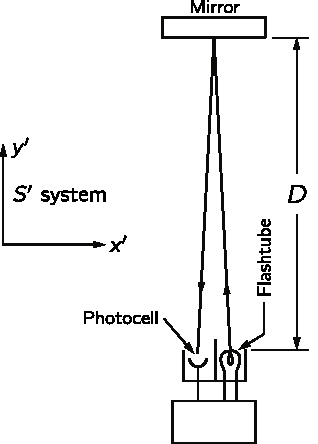
\includegraphics[width=0.4\linewidth]{fyz_fig003a.pdf}}
        \hspace{0.1\linewidth}                                                       &
        \subfloat[ ]{\label{fyz:fig003b}
          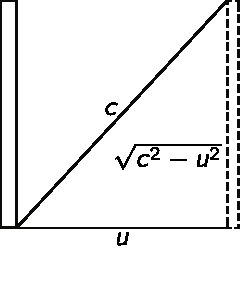
\includegraphics[width=0.25\linewidth]{fyz_fig003c.pdf}}                   \\
      \end{tabular}
      \begin{tabular}{c}
        \subfloat[ ]{\label{fyz:fig003c}
          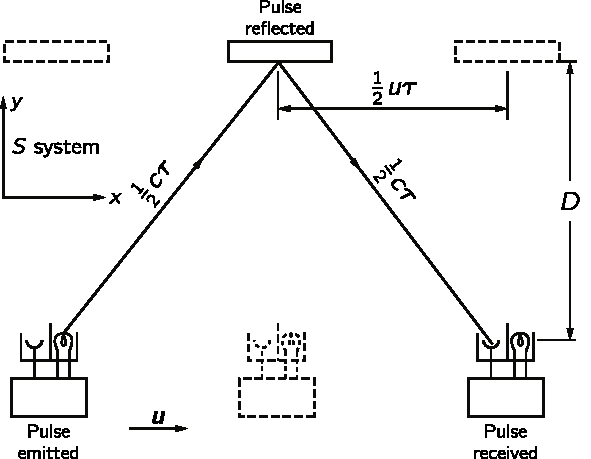
\includegraphics[width=0.9\linewidth]{fyz_fig003b.pdf}}
      \end{tabular}
      \caption{a) Světelné hodiny v klidu v soustavě \(S'\), b) Stejné hodiny v pohybující se 
               soustavě \(S\), c) Znázornění úhlopříčné dráhy světelného paprsku v pohybujících se
               světelných \uv{hodinách}
               (\cite[s.~217]{Feynman01})}
      \label{fyz:fig003}
    \end{figure}
    
    Velmi zajímavý příklad zpomalování času při pohybu poskytují \(\mu\) mezony (\emph{miony}). 
    Jsou to částice, které se spontánně rozpadají s průměrnou dobou života \SI{2.2e-6}{\s}. Na Zemi 
    se dostávají v kosmických paprscích a lze je i uměle vyrobit v laboratoři. Část z nich se 
    rozpadá ještě ve vzduchu, ale zbytek se rozpadne, jen co narazí na nějakou překážku a zastaví 
    se. Z krátké doby života mionu je jasné, že nemůže urazit dráhu mnohem delší než \num{600} 
    metrů, dokonce ani při rychlosti světla. Ale ačkoli miony vznikají ve vrchních vrstvách 
    atmosféry, asi ve výšce \num{10} kilometrů, přece je lze nalézt v kosmických paprscích v 
    pozemských laboratořích. Jak je to možné? Odpověď je taková, že různé miony se pohybují různou 
    rychlostí, některé z nich rychlostí blížící se rychlosti světla. Z jejich hlediska je doba 
    jejich života jen \num{2} mikrosekundy z našeho hlediska žijí podstatně déle - dostatečně 
    dlouho k tomu, aby se dostaly na povrch Země. Koeficient narůstání času jsme již uvedli a je 
    roven \(1/\sqrt{1 - u^2/c^2}\). Průměrná doba života mionů s různými rychlostmi byla dost 
    přesně změřena, přičemž výsledky jsou v dobrém souladu s tímto vztahem.
    
    Příčinu rozpadu mezonů neznáme, neznáme mechanizmus rozpadu, ale víme, že jejich chování je v 
    souladu s principem relativity. V tom spočívá užitečnost principu relativity - dovoluje nám 
    dělat předpovědi dokonce i o věcech, o kterých jinak mnoho nevíme. Například dříve, než bychom 
    vůbec věděli něco o tom, co způsobuje rozpad mezonů, můžeme předpovědět, že pohybuje-li se 
    rychlostí rovnou devíti desetinám rychlosti světla, pak zdánlivá doba jeho života
    je \(\num{2.2e-6}/\sqrt{1 - 9^2/10^2} = \SI{5.047e-6}{\s}\). Naše předpověď je správná - to je 
    to, co je na celé věci dobré.
    
  \section{Lorentzovská kontrakce}\label{fyz:IchapXVsecV}
    Vraťme se nyní k Lorentzově transformaci (\ref{FYZ:eq185}) a pokusme se lépe pochopit vztah 
    mezi souřadnicovými soustavami \((x,y, z, t)\) a \((x', y', z', t')\), které nazveme \(S\) a 
    \(S'\) nebo systémem Petra a Pavla. Již jsme si všimli, že první rovnice se zakládá na 
    Lorentzově návrhu kontrakce ve směru osy \(x\). Jak lze dokázat, že kontrakce skutečně nastává? 
    Nyní již chápeme, že podle principu relativity nemůže příčné rameno \(BC\) v 
    Michelsonově-Morleyově experimentu změnit svou délku; a přece nulový výsledek tohoto 
    experimentu vyžaduje rovnost časů. Aby měl experiment takovýto výsledek, podélné rameno \(BE\) 
    musí být kratší o faktor \(\sqrt{1 - u^2/c^2}\). Jak se projeví tato kontrakce v měřeních Petra 
    a Pavla? Předpokládejme, že Pavel se pohybuje v soustavě \(S'\) ve směru osy \(x\) a měří 
    metrovým pravítkem souřadnici \(x'\) nějakého bodu. Pravítko přiloží \(x'\)-krát, proto si 
    myslí, že měřená vzdálenost je \(x'\) metrů. Avšak z hlediska Petra, jenž je v soustavě \(S\), 
    se Pavlovo pravítko zkrátilo, takže skutečná vzdálenost je \(x'\sqrt{1 - u^2/c^2}\) metrů. 
    Jestliže se soustava \(S'\) vzdálila od soustavy \(s\) o vzdálenost \(ut\), pak pozorovatel v 
    soustavě \(S\) řekne, že v jeho souřadnicích má měřený bod vzdálenost \(x = x'\sqrt{1 - 
    u^2/c^2} + ut\), neboli
    \begin{equation*}
      x'= \frac{x-ut}{\sqrt{1 - \dfrac{u^2}{c^2}}}
    \end{equation*}
    což je vlastně první rovnice v Lorentzově transformaci.
    
  \section{Současnost}\label{fyz:IchapXVsecVI}
    Analogicky, z důvodů v rozdílnosti časové škály, má čtvrtá rovnice Lorentzovy transformace ve 
    jmenovateli stejný výraz. Nejzajímavější je v této rovnici člen \(ux/c^2\) v čitateli, neboť je 
    nový a neočekávaný. Jaký má smysl? Podíváme-li se pozorně na celou věc, zjistíme, že události, 
    které podle pozorování Pavla v soustavě \(S'\) nastanou současně na dvou různých místech, 
    \emph{nenastanou současně} podle Petrova pozorování v soustavě \(S\). Jestliže k jedné události 
    dojde v bodě \(x_1\), v okamžiku \(t_0\) a k druhé v bodě \(x_2\) a okamžiku \(t_0\) (tedy 
    současně), zjistíme, že dva odpovídající časy \(t_1'\) a \(t_2'\) se liší o
    \begin{equation*}
      t_1' - t_2'= \dfrac{\dfrac{u(x_1 - x_2)}{c^2}}{\sqrt{1 - \dfrac{u^2}{c^2}}}
    \end{equation*}
    Tento jev se nazývá „narušení současnosti nesoumístných událostí“. Abychom si ho objasnili, 
    uvažujme následující experiment.
    
    Předpokládejme, že kosmonaut si umístil hodiny na obou koncích kosmické lodi (soustava \(S'\)) 
    a chce se přesvědčit o tom, zda jsou hodiny navzájem synchronizovány. Jak lze hodiny 
    synchronizovat? Existuje k tomu mnoho způsobů. Jedním z nich, velmi nenáročným na výpočty, by 
    bylo nejprve určit bod přesně uprostřed mezi hodinami. Pak z něho vyslat světelný signál, který 
    se bude šířit oběma směry stejně rychle, takže obou hodin dosáhne současně. Tento současný 
    příchod obou signálů lze použít k synchronizování hodin. Předpokládejme, že hodiny v soustavě 
    \(S'\) budou sesynchronizovány touto metodou. Podívejme se, zda pozorovatel v systému \(S\) 
    bude souhlasit, že oboje hodiny jsou synchronizovány. Kosmonaut v soustavě \(S'\) má právo 
    věřit, že jsou synchronizovány, neboť neví, že se pohybuje. Ale pozorovatel v soustavě \(S\) 
    tvrdí, že protože se loď pohybovala, přední hodiny ubíhaly před signálem, a světlo tedy muselo 
    urazit větší dráhu, než je poloviční vzdálenost mezi hodinami a zadní hodiny se pohybovaly 
    naproti signálu, takže tato vzdálenost byla kratší. Proto signál dosáhl zadních hodin dříve, 
    ačkoli si kosmonaut myslel, že oba signály došly současně. Vidíme tedy, že jestliže si 
    kosmonaut myslí, že události na dvou různých místech jsou současné, musí \emph{stejným} 
    hodnotám času \(t'\) v jeho souřadnicové soustavě odpovídat dvě \emph{různé} hodnoty \(t\) v 
    druhé souřadnicové soustavě!
    
  \section{Čtyřvektory}\label{fyz:IchapXVsecVII}
    Podívejme se, co ještě můžeme objevit v Lorentzově transformaci. Je zajímavé, že transformace 
    \(x\) a 
    \(t\) má podobný tvar jako transformace \(x\) a \(y\) při rotaci souřadnic v kapitole 
    \ref{chap:fey_vektor}. Tam jsme měli
    \begin{align}
       x' &= x\cos\vartheta + y\sin\vartheta             \nonumber \\
       y' &= y\cos\vartheta - x\sin\vartheta             \label{FYZ:eq190}`
    \end{align}
    tj., nové \(x'\) je kombinací starého \(x\) a \(y\) a stejně tak nové \(y'\) je kombinací 
    starého \(x\) a \(y\). Podobně tomu je v Lorentzově transformaci, kde nové \(x'\) vzniká 
    zkombinováním \(x\) a \(t\) a nové \(t'\) je kombinací \(t\) a \(x\). Takže Lorentzova 
    transformace je analogická rotaci, pouze je to „rotace“ v \emph{prostoru a čase}, což se zdá 
    být podivné. Tuto analogii lze prověřit, vypočteme-li veličinu
    \begin{equation}\label{FYZ:eq191}
      x'^2 + y'^2 + z'^2 -c^2t'^2 = x^2 + y^2 + z^2 - c^2t^2.
    \end{equation}
    První tři členy na každé straně této rovnice dávají v trojrozměrné geometrii \emph{druhou 
    mocninu vzdálenosti bodu od počátku (povrch koule)}, jenž se nemění (je invariantní) vzhledem k 
    rotaci souřadnicových os. Podobné z rovnice (\ref{FYZ:eq191}) vyplývá, že existuje taková 
    kombinace souřadnic, včetně času, která je invariantní vzhledem k Lorentzové transformaci. To 
    znamená, že analogie s rotacemi je úplná a je takového druhu, že vektory, tj. veličiny 
    sestávající ze „složek“, které se transformují podobné jako souřadnice a čas, jsou užitečné i 
    ve spojení s relativitou.
    
    Tak se dostáváme k rozšíření pojmu vektor, jenž měl doposud jen prostorové složky, a to tak, že 
    mu přidáme časovou složku. To znamená, že předpokládáme existenci vektorů se čtyřmi slož¬kami, 
    z nichž tři jsou jako složky obyčejného vektoru, k nimž je připojena čtvrtá složka - analog 
    času.
    
    V následujících kapitolách provedeme hlubší analýzu této koncepce. Zjistíme, že aplikujeme-li 
    myšlenky tohoto paragrafu na hybnost, příslušná transformace bude mít tři prostorové části - 
    podobné složkám obyčejné hybnosti a čtvrtou - časovou složku, jíž je \emph{energie}.
     
  \section{Relativistická dynamika}\label{fyz:IchapXVsecVIII}
    Nyní jsme připraveni, abychom z obecnějšího hlediska přezkoumali, jaký tvar mají zákony 
    mechaniky při Lorentzové transformaci. (Zatím jsme si vysvětlili, jak se mění délka a čas, ale 
    ještě jsme si nevysvětili, jak dostáváme modifikovaný vztah pro \(m\), rovnici 
    (\ref{FYZ:eq182}). Vysvětlíme si to v další kapitole.) Abychom viděli, jaké jsou důsledky 
    Einsteinovy úpravy \(m\) v Newtonově mechanice, vezměme si nejdříve Newtonův zákon, že síla je 
    rovna změně hybností
    \begin{equation}\label{FYZ:eq192}
      \vec{F} = \der{m\vec{v}}{t}.
    \end{equation}
    Hybnost je rovna \(m\vec{v}\) jako předtím, ale pro nové \(m\) platí
    \begin{equation}\label{FYZ:eq193}
      \vec{p} = m\vec{v} = \frac{m_0\vec{v}}{\sqrt{1-\dfrac{v^2}{c^2}}}.
    \end{equation}
    
    To je Einsteinova úprava Newtonových zákonů. Při této úpravě, jsou-li si akce a reakce stále 
    rovny (což nemusí platit v každé chvíli, ale v dlouhodobém průměru to platí), bude se hybnost 
    zachovávat podobně jako předtím, ale veličina, která se zachovává, není \(m\vec{v}\) s 
    konstantní hmotností, ale je to veličina ze vztahu (\ref{FYZ:eq193}) s modifikovanou hmotností. 
    Jestliže ve vztahu pro hybnost provedeme tuto záměnu, bude se hybnost stále zachovávat.
    
    Nyní si všimněme, jak se mění hybnost v závislostí na rychlosti. V Newtonově mechanice je 
    úměrná rychlosti a podle (\ref{FYZ:eq193}) to platí i v relativistické mechanice v poměrně 
    velkém rozsahu rychlostí, jež jsou malé ve srovnání s \(c\), neboť výraz s odmocninou se liší 
    od \(1\) jen velmi málo. Ale pro \(v\) téměř rovno \(c\) se výraz s odmocninou blíží k nule a 
    hybnost proto narůstá do nekonečná. 
    
    Co se bude dít, jestliže po dlouhou dobu bude na těleso působit konstantní síla? V newtonovské 
    mechanice nabírá těleso rychlost a jeho rychlost narůstá i po dosažení rychlosti světla. V 
    relativistické mechanice to není možné. V teorii relativity nabývá těleso stále větší hybnosti, 
    ne rychlosti. Jeho hybnost může spojitě narůstat, neboť narůstá jeho hmotnost. Po nějakém čase 
    se pohyb tělesa prakticky nezrychluje, ale jeho hybnost se dále zvětšuje. Jestliže se pod 
    vlivem síly změní rychlost nějakého tělesa velmi málo, z toho přirozeně vyplývá, že těleso má 
    velkou setrvačnou hmotnost. Ale přesně to potvrzuje náš vztah pro výpočet relativistické 
    hmotnosti (podívejte se na vztah \ref{FYZ:eq193}) - tvrdí, že hmotnost je velmi velká pro \(v\) 
    přibližně stejné jako \(c\). Uveďme příklad. K vychýlení rychle letících elektronů v 
    synchrotronu Kalifornského technického institutu potřebujeme \num{2000}-krát silnější 
    magnetické pole, než by se dalo očekávat na základě Newtonových zákonů. To znamená, že hmotnost 
    elektronů v synchrotronu je \num{2000}-krát větší než jejich normální hmotnost a je rovna 
    hmotnosti protonu! Aby \(m\) bylo \num{2000}-krát větší než \(m_0\), musí být \(1 - v^2/c^2\) 
    rovno \num{1/4 000 000}, což znamená, že \(v^2/c^2\) se liší od \num{1} jen o \num{1/4 000 
    000}, nebo že v se liší od \(c\) jen o \num{1/8 000 000}, a tak se rychlost elektronů blíží 
    rychlosti světla. Kdyby elektrony a světlo vyletěly současně ze synchrotronu, co by doletělo 
    dříve do Bridge Lab (vzdálenost asi \num{230} metrů)? Samozřejmě, že světlo, neboť světlo je 
    vždy rychlejší\footnote{Závody s viditelným světlem by ve skutečnosti vyhrály elektrony díky 
    indexu lomu vzduchu. Paprsky \(\gamma\) by si však vedly lépe.}. O kolik dříve? O jakou dobu 
    dříve, to lze říci velmi obtížně, můžeme ale říci, o jakou vzdálenost předběhne světlo 
    elektrony. Je to asi \SI{1/40}{\mm}, nebo \num{1/4} tloušťky papíru! Elektrony pohybující se 
    takovou rychlostí mají obrovskou hmotnost, ale jejich rychlost nemůže převýšit rychlost světla.
    
    Podívejme se nyní na další důsledky relativistické změny hmotnosti. Představme si pohyb molekul 
    plynu v uzavřené nádobě. Zahříváním plynu se zvyšuje rychlost pohybu molekul, a tedy i jejich 
    hmotnost, a plyn je těžší. Přibližný vzorec k vyjádření přírůstku hmotnosti můžeme pro případ 
    malých rychlostí najít pomocí rozvoje
    \begin{equation*}
      \frac{m_0}{\sqrt{1-\frac{v^2}{c^2}}} = m_0\left(1-\frac{v^2}{c^2}\right)
    \end{equation*}
    do mocninné řady použitím \emph{Newtonova binomického rozvoje}.
    Dostáváme
    \begin{equation*}
      m_0\left(1-\frac{v^2}{c^2}\right) 
        = m_0\left(1 + \frac{1}{2}\frac{v^2}{c^2} + 
                       \frac{3}{8}\frac{v^4}{c^4} + \ldots \right)
    \end{equation*}
    Odtud je jasně vidět, že pro malá \(v\) řada velmi rychle konverguje, a další členy následující 
    za druhým nebo třetím členem jsou zanedbatelně malé. Proto můžeme psát, kde druhý člen na pravé 
    straně vyjadřuje přírůstek hmotnosti způsobený rychlostmi molekul. 
    \begin{equation}\label{FYZ:eq194}
      m = m_0 + \frac{1}{2}m_0v^2\left(\frac{1}{c^2}\right),
    \end{equation}
    kde druhý člen na pravé straně vyjadřuje přírůstek hmotnosti způsobený rychlostmi molekul. Se 
    stoupající teplotou úměrně narůstá \(v^2\). Lze tedy říci, že přírůstek hmotnosti je úměrný 
    přírůstku teploty. Protože \(1/2m_0v^2\) je ve starém Newtonově smyslu kinetická energie, 
    můžeme říci, že přírůstek hmotnosti plynu je roven přírůstku kinetické energie dělenému 
    \(c^2\), nebo že \(\Delta m = \Delta(W_k)/c^2\).
    
  \section{Ekvivalence hmotnosti a energie}\label{fyz:IchapXVsecIIX}
    Uvedená skutečnost vedla Einsteina k nápadu, že jestliže hmotnost tělesa je rovna celkové 
    energii dělené \(c^2\), pak hmotnost tělesa lze vyjádřit jednodušším vztahem, než je 
    (\ref{FYZ:eq182}). Když (\ref{FYZ:eq194}) vynásobíme \(c^2\), máme
    \begin{equation}\label{FYZ:eq195}
      mc^2 = m_0c^2 + \frac{1}{2}m_0v^2 + \ldots,
    \end{equation}
    Výraz na levé straně vyjadřuje celkovou energii tělesa a v posledním členu poznáváme obyčejnou 
    kinetickou energii. Velký konstantní výraz \(m_0c^2\) Einstein interpretoval jako část celkové 
    energie tělesa, jako vnitřní energii známou pod názvem \emph{„klidová energie“}.
    
    Zjistíme, jaké jsou důsledky toho, když spolu s Einsteinem předpokládáme, že \emph{energie 
    tělesa je vždy rovna \(mc^2\)}. Jako zajímavý důsledek odvodíme vztah ((\ref{FYZ:eq182})) 
    závislosti hmotnosti na rychlosti, který jsme doposud jen předpokládali. Nechť je těleso 
    zpočátku v klidu. Jeho energie je \(m_0^c2\). Pak necháme na těleso působit sílu, jež ho uvede 
    do ohybu a dodá mu kinetickou energii. Protože se zvýšila jeho energie, zvýšila se i jeho 
    hmotnost - to vyplývá z původního předpokladu. Dokud působí síla, tak oboje, energie i 
    hmotnost, stále rostou. V kapitole \ref{fyz:chap_fey_work} jsme uvedli, že změna energie s 
    časem je rovna součinu síly a rychlosti, tedy
    \begin{equation}\label{FYZ:eq196}
      \der{E}{t} = \vec{F}\cdot\vec{v}
    \end{equation}
    Kromě toho \(F=\der{(mv)}{t}\) (kapitola \ref{fyz:IchapIX}, vztah \ref{fyz:eq052}). 
    Spojíme-li tyto vztahy s definicí \(E\), máme z \ref{FYZ:eq196}
    \begin{equation}\label{FYZ:eq197}
      \der{(mc^2)}{t} = \vec{v}\cdot\der{(m\vec{v})}{t}
    \end{equation}
    Tuto rovnici chceme řešit vzhledem k \(m\). Nejprve vynásobíme obě strany \(2m\), čímž se 
    rovnice změní na
    \begin{equation}\label{FYZ:eq198}
      c^2(2m)\der{m}{t} = 2m\vec{v}\cdot\der{(m\vec{v})}{t}
    \end{equation}
    Nyní se potřebujeme zbavit derivací, čehož dosáhneme integrací obou stran. Veličina \((2m) 
    dm/dt\) je derivací \(m^2\) podle času a \((2m\vec{v})\cdot d(m\vec{v})/dt\) je derivací 
    \((mv^2)\) podle Času. Takže rovnice (\ref{FYZ:eq198}) je stejná jako rovnice 
    \begin{equation}\label{FYZ:eq199}
      c^2\der{m^2}{t} = \der{(m^2v^2)}{t}
    \end{equation}
    Když jsou si derivace dvou veličin rovny, pak se tyto veličiny liší nanejvýš o konstantu. 
    Označme ji \(C\). Můžeme proto psát
    \begin{equation}\label{FYZ:eq200}
      m^2c^2 = m^2v^2 + C.
    \end{equation}
    Konstantu \(C\) potřebujeme určit přesněji. Protože (\ref{FYZ:eq200}) platí pro všechny 
    rychlosti, můžeme zvolit případ \(v = 0\) a odpovídající hmotnost označit \(m_0\). Dosazením 
    těchto hodnot do (\ref{FYZ:eq200}) máme
    \begin{equation}\label{FYZ:eq201}
      m_0^2c^2 = 0 + C.
    \end{equation}
    Tuto hodnotu \(C\) můžeme nyní dosadit do rovnice (\ref{FYZ:eq200}), která bude mít tvar
    \begin{equation}\label{FYZ:eq202}
      m^2c^2 = m^2v^2 + m_0^2c^2.
    \end{equation}
    Dělením \(c^2\) a úpravou dostaneme
    \begin{equation*}
      m^2\left(1-\dfrac{v^2}{c^2}\right) = m_0^2,
    \end{equation*}
    odkud máme
    \begin{equation}\label{FYZ:eq203}
      \boxed{m = \dfrac{m_0}{\sqrt{1-\dfrac{v^2}{c^2}}}}\,.
    \end{equation}
    To je vztah (\ref{FYZ:eq182}) a vyjadřuje přesně to, co je třeba aby v rovnici 
    (\ref{FYZ:eq195}) souhlasila hmotnost a energie.
    
    Za obvyklých podmínek představují změny energie jen velmi malé změny hmotnosti. Je to dáno tím, 
    že většinou nedokážeme uvolnit mnoho energie z daného materiálu, ale například u atomové bomby 
    s explozivní silou ekvivalentní dvaceti kilotunám TNT lze ukázat, že při uvolnění energie jsou 
    zplodiny po výbuchu o \num{1} gram lehčí, než počáteční hmotnost reagující látky, tj. uvolněná 
    energie má podle vztahu \(\Delta E=\Delta(mc^2)\) hmotnost \num{1} gram. Teorie ekvivalence 
    hmotnosti a energie byla nádherně ověřena experimenty, při nichž látka anihilovala - přeměnila 
    se úplně na energii. Při nich elektron a jeho částice, pozitron, interagují v klidu, přičemž 
    každý z nich má klidovou hmotnost. Jakmile se přiblíží, obě částice zmizí a vzniknou dva gama 
    paprsky, každý s energií \(m_0c^2\). Tento experiment nám umožňuje přímo určit energii spojenou 
    s existencí klidové hmotnosti částice.
    
    
  \section{Příklady a cvičení}\label{fyz:IchapXVsecIX}

} %tikzset
%---------------------------------------------------------------------------------------------------
\printbibliography[heading=subbibliography]
\addcontentsline{toc}{section}{Seznam literatury}